
\subsection{Answers}
\begin{table}[htb]%
\begin{center}%
\caption{Q21: In most of your programs, do you pack MPI function calls into their own file or files to have your own abstraction layer for communication?}%
\label{tab:Q21-ans}%
\begin{tabular}{l|l|r}%
\hline%
Choice & Abbrv. & \# Answers \\%
\hline%
{\small Yes, to minimize the changes of communic$\cdots$} & Yes & 331 (40.0\%) \\%
{\small Yes, but I have no special reason for do$\cdots$} & Yes, but no reason & 60 (7.2\%) \\%
No, my program is too small to do that. & No, too small & 122 (14.7\%) \\%
{\small No, MPI calls are scattered in my programs.} & No, scattered & 276 (33.3\%) \\%
other & - & 39 (4.7\%) \\%
\hline%
\multicolumn{2}{c}{total} & 828 \\%
\hline%
\end{tabular}%
\end{center}%
\end{table}%


\subsection{List of other answers}
\begin{itemize}
\item Europe:France: I am not the main architect of the codes, so I do the same as what is already done
\item Europe:France: I tried to, but such a design is not always easy to implement efficiently without losing too much in readablity
\item Europe:France: It clearly depends of targeted software, but I tend to write my own abstration layer
\item Europe:France: It's a mix of both, I try to keep the communications part as a separate layer whenever I can.
\item Europe:France: Mostly use through libraries
\item Europe:France: Through Boost MPI
\item Europe:France: Yes so that other non-mpi part developers does not get bothered by mpi functions
\item Europe:France: Yes, I have few MPI function call into my program(s), and we use an other library which does most of the MPI function calls
\item Europe:Germany: I do not call MPI routines
\item Europe:Germany: I'm mainly adapting existing code
\item Europe:Germany: Make standard operations easier
\item Europe:Germany: No, but i would like to implement it if i had more time for code improvement
\item Europe:Germany: Partially encapsulated to allow for changes of communication patterns, but otherwise MPI calls scattered throughout the application (only few calls, though).
\item Europe:Germany: Partly
\item Europe:Germany: Sometimes, to make code more readable
\item Europe:Germany: Using boost::mpi
\item Europe:Germany: YES, to switch between SEQUENTIAL und MPI
\item Europe:Germany: Yes, using templates for type safety and for transportation of own classes
\item Europe:Italy: not sure
\item Europe:UK: I pack elementary vector operations into their own files. In turn, those are small enough to call MPI directly.
\item Europe:UK: Mixed, some are abstracted some are direct MPI calls
\item Europe:UK: Sometimes, for the same reasons as subroutines in general
\item Europe:UK: Yes, to abstract interfaces to 32-bit/64-bit libraries
\item Europe:UK: Yes, to allow a serial implementation of the application when MPI is not readily  available
\item Europe:UK: Yes, to allow users to easily compile without MPI parallelism on certain platforms
\item Europe:UK: Yes, to reduce API complexity
\item Europe:UK: Yes, to simplify the code for other developers, who are often not software specialists
\item Europe:others: 1) I make a special Fortran library (low level abstraction) 2) Create Scheme macros that do different things depending on the type of parellisation needed (high level abstraction)
\item Europe:others: I do not write programs
\item Europe:others: I either work on some one else large code base or my own simple tests/examples/proxies. My code is usually single file.
\item Europe:others: I/we use Python/C, and I/we mostly use Python bindings for MPI calls (not mpi4py though, for historical reasons)
\item Europe:others: It's a mix depending on how essential the MPI functionality is for the routine in question.
\item Europe:others: Yes, but the abstraction is so leaky, I couldn't replace the communication layer
\item Europe:others: Yes, to extend the abstraction provided by MPI.
\item Europe:others: Yes, to keep the numerical algorithm implementation separated from MPI communication.
\item Europe:others: no
\item Japan: I don't know.
\item Russia: Sometimes, to simplify and unify (in non MPI mode) communications
\item USA: It depends on the program;my longer programs have abstraction layers but shorter ones do not

\end{itemize}

This question relates on how developers do program their MPI applications. 

In one third of the cases, MPI calls are put in a special file to better manage
where the communication between processes are done and another one third says that
MPI called are scattered in the program even if the program is large enough. It
seems there is no specific ways of programming in MPI. 

\begin{figure}[htb]
\begin{center}
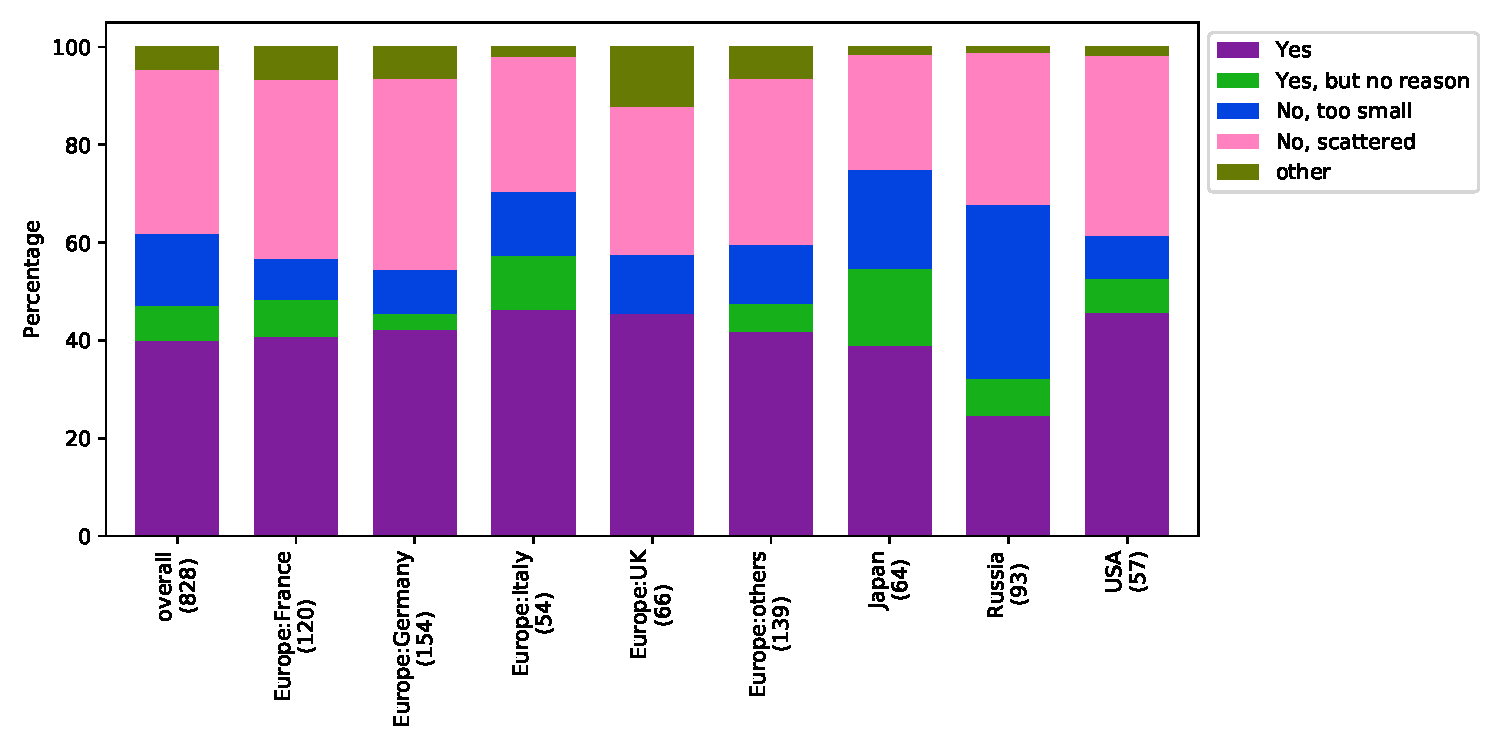
\includegraphics[width=10cm]{../pdfs/Q21.pdf}
\caption{Simple analysis: Q21}
\label{fig:Q21}
\end{center}
\end{figure}



It is very interesting that the asnwder of program is 'too small' in
Russia dominates, while the asnwers of 'packing' and 'scattered'
equally dominate in the other countries. 
